\documentclass[a4paper]{report}
%\usepackage[french]{babel}
\usepackage[utf8]{inputenc}
\usepackage[]{amsmath}
\usepackage[]{braket} % \bra, \ket etc
\usepackage{graphicx}
\usepackage{tikz}
\usepackage{subcaption} % package pour faire des subfigures
\usepackage{multirow} % package pour multirow/multicolumn
\usepackage{booktabs} % package pour top/mid/bottom rule
\usepackage{empheq} % Tout ca pour encadrer des équations
\usetikzlibrary{optics}
\usetikzlibrary{shapes}
\usetikzlibrary{fit}

\title{Titre}
\author{Clément Pellet-Mary}
\date\today

\begin{document}
\chapter{Système à deux niveaux}
  \section{Représentation, sphère de Bloch}
  \begin{figure}[h]
  \centering
  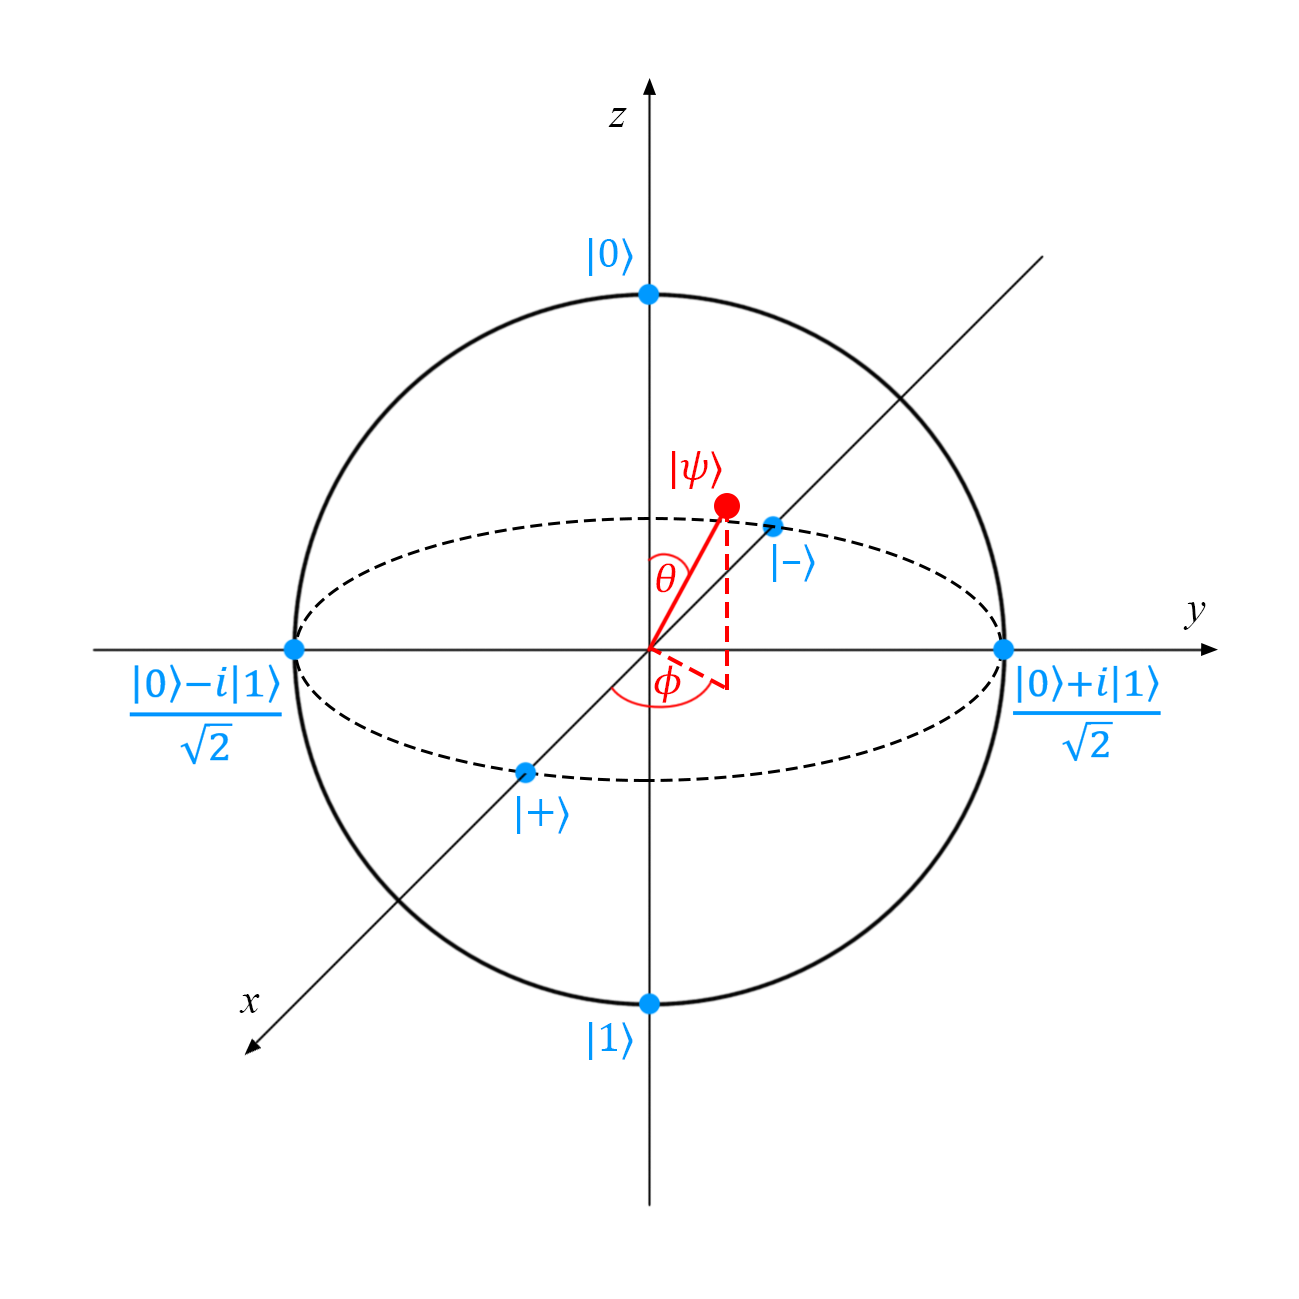
\includegraphics[width=.8\textwidth]{BlochSphere}
  \caption{$\ket{\psi}=\cos (\theta/2)\ket{0}+\sin (\theta/2)e^{i \phi} \ket{1}$}
  \end{figure}
  
  On va prendre le formalisme des spins (qui ne correspond pas au dessin mais bon). 
  
  Ta base de base va être $\{\ket{-},\ket{+}\}$, les vecteurs propres de $S_z$, et
  \begin{itemize}
  \item $\ket{+}_x=\dfrac{\ket{+}+\ket{-}}{\sqrt(2)} \quad \ket{-}_x=\dfrac{\ket{+}-\ket{-}}{\sqrt(2)}$
  \item $\ket{+}_y=\dfrac{\ket{+}+i\ket{-}}{\sqrt(2)} \quad \ket{-}_y=\dfrac{\ket{+}-i\ket{-}}{\sqrt(2)}$
  \end{itemize}
  
  
  Avec $S_x= \begin{pmatrix} 0 & 1 \\ 1 & 0  \end{pmatrix}$ et $S_y= \begin{pmatrix} 0 & -i \\ i & 0  \end{pmatrix}$
  
  Pour un vecteur quelconque sur la sphère de Bloch (état pur), \begin{equation}
  \ket{\psi}=\cos (\theta/2)\ket{+}+\sin (\theta/2)e^{i \phi} \ket{-}
  \end{equation}
  
  Le truc à retenir c'est que $\ket{\psi}$ est le vecteur $\ket{+}_\textbf{u}$où $\textbf{u}$ est la direction dans la sphère de Bloch.
  
  \section{Évolution d'un système pur à 2 niveaux}
  Ton Hamiltonien va être typiquement de la forme $H=H_0 +H_1$ avec
  \begin{itemize}
  \item $H_0=\hbar \begin{pmatrix} -\omega_0/2 & 0 \\ 0 & \omega_0/2  \end{pmatrix}$ (l'ordre de la base c'est $\{\ket{-},\ket{+}\}$). Pour un spin, ca va venir du champ magnétique selon z : $-M.B_0$, donc $\omega_0=\gamma B_0$. Dans le cas d'un atome c'est simplement le niveau d'énergie de l'électron.
  \item $H_1$ est le terme de couplage, dont on ne retiendra que les termes non-diagonaux. On traitera une perturbation statique, et une perturbation (quasi)résonnante à $\omega_0$ (Rabi).
  \end{itemize}
   \subsection{Perturbation statique : anti-croisement}
   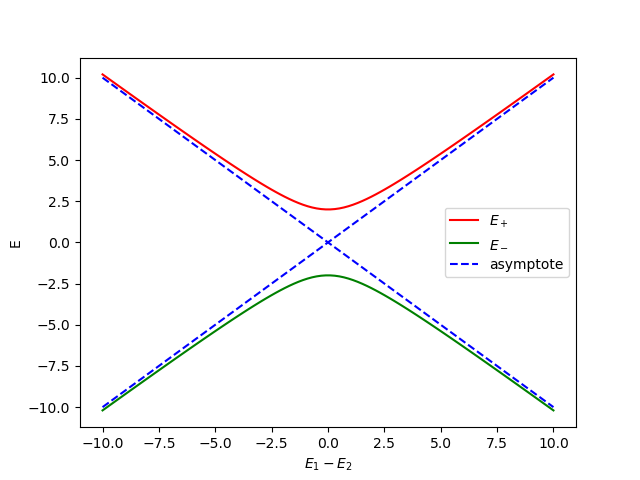
\includegraphics[width=\textwidth]{anti_croisement}
   
   Hamiltonien indépendant du temps, on diagonalise. $E_1$ et $E_2$ sont les énergies propres de $H_0$, $E_\pm$ celles de  $H= \begin{pmatrix} E_1 & W_{12} \\ W_{21} & E_2  \end{pmatrix}$
   
   On trouve : \begin{align}  
   E_\pm &= \dfrac{E_1-E_2}{2}\pm\dfrac{1}{2}\sqrt{(E_1-E_2)^2+4|W_{12}|^2} \\   
   \ket{\psi_+} &= \cos \dfrac{\theta}{2} e^{-i\phi/2} \ket{\psi_1}+\sin \dfrac{\theta}{2} e^{i\phi/2} \ket{\psi_2} \\   
   \ket{\psi_-}&= -\sin \dfrac{\theta}{2} e^{-i\phi/2} \ket{\psi_1}+\cos \dfrac{\theta}{2} e^{i\phi/2} \ket{\psi_2} 
  \end{align}
   
   Avec $\tan \theta = 2 \dfrac{|W_{12}|}{E_1-E_2}$ et $W_{12}=e^{i\phi}|W_{12}|$
   
   En particulier, on voit que pour 2 niveaux dégénérés, le fait qu'il existe un couplage entre les deux va lever la dégénérescence, et créer un état de plus basse énergie, donc plus stable (d'où la stabilité des cycles aromatiques, genre benzène).
   
   \subsection{Perturbation sinusoïdale : Rabi}
   La perturbation peut être un champ magnétique transverse oscillant à $\omega$ pour un spin, une onde électromagnétique pour un système atomique, ou n'importe quel couplage sinusoïdal ne faisant intervenir que des termes hors-diagonaux.
   
   Remarque pour le couplage lumière-matière, c'est parce que l'opérateur dipôle $\textbf{D}=q\textbf{r}\begin{pmatrix}
   0 & d \\ d^* & 0
   \end{pmatrix}$ n'a pas de termes diagonaux, car les états propres du système ont une parité définie (pas de sens privilégié, symétrie centrale).
   
   On a alors \begin{equation}
    H=\dfrac{\hbar}{2} \begin{pmatrix} \omega_0 & \omega_1 e^{-i\omega t} \\ \omega_1 e^{i\omega t} & -\omega_0  \end{pmatrix}
\end{equation}    où $\omega_1$ correspond à l'intensité du couplage, et $\omega$ la pulsation de l'oscillation.
   
   On va passer dans le référentiel tournant par la transformation \begin{equation}
   U=\begin{pmatrix} e^{i\omega t/2} & 0 \\ 0 & e^{-i\omega t/2}  \end{pmatrix}
   \end{equation}On fait également l'approximation de l'onde tournante : Rotating wave / secular approx, pour virer le terme en $2\omega$. Le résultat n'est donc valable que proche de la résonance 
   
   $H$ devient alors \begin{equation}
   \tilde{H}=\dfrac{\hbar}{2} \begin{pmatrix} -\Delta\omega & \omega_1  \\ \omega_1 & \Delta\omega  \end{pmatrix}
   \end{equation} (A revoir) qui est indépendante du temps, donc on résout, on repasse dans le référentiel classique et on trouve que, pour un état initialement en $\ket{+}$, la probabilité de passage dans l'état $\ket{-}$ vaut : \begin{equation}
   \mathcal{P}_{+-}(t)=\dfrac{\omega_1^2}{\omega_1^2+(\Delta\omega)^2}\sin^2(\sqrt{\omega_1^2+(\Delta\omega)^2}\dfrac{t}{2})
   \end{equation}
   On retrouve l'évolution temporelle, sinusoïdale à la fréquence de Rabi $\Omega=\sqrt{\omega_1^2+(\Delta\omega)^2}$ (le /2 vient du fais que tu as un sinus carré, qui oscille donc deux fois plus vite qu'un sinus normal. Tu fais donc une période en $2\pi/\Omega$.)
   
   On retrouve également la Lorentzienne pour l'amplitude maximale en fonction du désaccord.
   
   \subsection{Franges de Ramsey}
   Le but ici ça va être de mesurer la fréquence d'une transition. Jusque là assez classique en spectro. Une méthode pour ça, c'est de se fixer un temps $\tau$, et de choisir $\Omega$ pour avoir une pulse $\pi$, soit $\Omega=\pi/\tau$. Tu vas ensuite scanner en fréquence ton laser résonnant : tu vas mesurer une lorentzienne de largeur $\Omega \approx 1/\tau$. Donc pour avoir une mesure précise, il te faut $\tau$ le plus grand possible. Ca c'est Fourier/Heinsnberg temps/énergie. Sauf que pour un temps long, bah t'as l'émission spontanée qui vient t'emmerder. D'où le lifetime-limited. Et bah Ramsay c'est exactement les mêmes limitations, mais c'est plus pratique dans certains cas visiblement.
   
   Ramsey, lui, c'est la fameuse méthode des 2 pulses $\pi/2$ : 2 pulses identiques (avec la même phase !) très courte (durée $t$) et séparée d'un temps long ($T >> t$).
   
   Le mieux c'est de se représenter ça graphiquement : ton laser est légèrement detuné, à la fréquence $\omega$. Tu vas imaginer ta sphère de Bloch dans le référentiel tournant à $\omega$. A cause du detuning, elle tourne (lentement). Comme les pulses sont très rapides, tu vas négliger la rotation pendant la durée des pulses (ce qui revient à dire que les pulses ont un spectre très large, donc forcément résonnant). La population de l'état excité (proportionnelle à la fluorescence) après la deuxième pulse est donc \begin{equation}
   p_e=\dfrac{1}{2}(1+\cos\Delta T)
   \end{equation}
   Tu as donc un résultat aussi précis que si tu avais réalisé une pulse $\pi$ de durée $T$.
   
   Pour l'appellation "Interférométre de Ramsay" ou "Franges de Ramsay", c'est parce que tu as un processus d'interférence type Mach-Zender, où les séparatrices sont tes pulses, et les deux voies possibles pour passer du fondamental à l'état excité viennent du fait que tu peut être excité à la première ou à la deuxième pulse, et ces deux chemins peuvent être constructifs ou destructifs.
   
   Pour la résolution, c'est celle d'un interferomètre à deux voies : \begin{equation}
   \delta_{min}=\dfrac{\sqrt{2}}{T\sqrt{N}}
   \end{equation}
   où $N$ est le nombre d'atomes sondés.
   
   \section{Système impur : Optical Bloch Equations}
   
   \subsection{Origine de l'impureté et approximations du modèle}
   On considère qu'un système est impur à partir du moment où il est couplé à un autre système qu'on ne veut/peut pas décrire (à savoir "l'environnement"). Dans ce cas on fait une réduction du système total en "traçant" sur l'environnement.
   
   Dans le cas qui nous intéresse ici, on va considérer notre système à 2 niveaux couplé à un reversoir (à savoir le vide et tout ses modes) qui vérifie ces deux hypothèses :\begin{itemize}
   \item \textbf{Born approximation} : On ne garde le terme d'interaction entre le système et l'environnement qu'à l'ordre le plus faible. D'après J-M Raymond ça signifie que toute perturbation du système envoyée au réservoir est "perdue".
   \item \textbf{Markov approximation} : Le réservoir n'a pas de mémoire, ou bien encore, dans la représentation de Heisenberg, que les observables du réservoir un temps de corrélation extrêmement court (de l'ordre de $\tau_c \approx 10^{-15} s$, c'est à dire la fréquence caractéristique des modes qui nous intéressent).
   \end{itemize}
   \subsection{Dérivation des OBE}
   On va considérer 3 phénomènes : \begin{itemize}
   \item L’interaction cohérente (donc évolution Hamiltonienne) avec le champ quasi-résonnant. On se place dans la représentation en interaction, et H s'écrit \begin{equation}
   H=-\dfrac{\hbar \Delta }{2} \sigma_z + \dfrac{\hbar \Omega}{2} \left( \sigma_+ e^{i\phi} + \sigma_- e^{-i\phi} \right)
   \end{equation}
   Avec $\Delta = \omega - \omega_{eg}$, $\Omega = -\dfrac{d\cdot E_0}{\hbar}$ et l'amplitude complexe du champ s'écrit  \begin{equation}
   E_1=E_0 e^{i\phi}
   \end{equation}
   \item La relaxation due à l'émission spontanée (jump operator $\sigma^-$ et temps caractéristique $T_1$)
   \item Le phase damping/pure dephasing du aux fluctuations locales du champ électrique/magnétique qui vont faire varier les niveaux d'énergie (par effet Stark / Zeeman) et provoquer un déphasage entre les deux états, mais sans modifier les populations (à creuser un peu).
   
   Le déphasage maximum éant un déphasage de $\pi$ entre les deux états, le jump operator qu'on va considérer est tout simplement $\sigma_z$, et le temps caractéristique associé est $T_2$
\end{itemize}      

Dans ces conditions, on met tout ça dans le Lindbaldien et on résout. On trouve finalement les OBE : 
\begin{empheq}[box=\fbox]{align}
\dfrac{d \, \rho_{ee}}{dt} &= \dfrac{d}{\hbar} \mathrm{Im} (\rho_{eg} E_1^*) - \Gamma \rho_{ee} \\ 
\dfrac{d \, \rho_{eg}}{dt} &= i\Delta \rho_{eg} -i\dfrac{d}{2\hbar} E_1(\rho_{ee}-\rho_{gg}) - \gamma ' \rho_{eg}
\end{empheq}

Avec \begin{equation}
\gamma ' = \gamma + \dfrac{\Gamma}{2}
\end{equation}

Ou encore \begin{equation}
\dfrac{1}{T_2^*} = \dfrac{1}{T_2} + \dfrac{1}{2T_1}
\end{equation}

Remarque : le $\Gamma/2$ pour les cohérences il vient directement des termes en $-\dfrac{1}{2} L^\dagger_\mu L_\mu \rho$ et $-\dfrac{1}{2} \rho L_\mu^\dagger L_\mu $ dans le Lindbladien.
   \subsection{Autre formulations}
   \subsubsection{Vecteur de la sphère de Bloch}
   Soit la matrice densité : 
   \begin{equation}
   \rho=\begin{pmatrix}
   \rho_{ee} & \rho_{eg} \\ \rho_{ge} & \rho_{gg}
   \end{pmatrix}
   \end{equation}
   Avec $\rho_{ee}+\rho_{gg}=1$ et $\rho_{eg}=\rho_{ge}*$ donc 3 paramètres libres, on va donc réécrire  \begin{equation}
   \rho=\dfrac{1}{2}\begin{pmatrix}
   1+Z & X-iY \\ X+iY & 1-Z
   \end{pmatrix}
   \end{equation}
   Il se trouve que $X,Y$ et $Z$ sont les coordonnées de ton vecteur dans la sphère de Bloch. Plutôt pratique, et ça te donne une contrainte graphique sur tes cohérences.
   
 
  \end{document}	
  
  